\subsection{Benötigte Register}
Um das Programm zu entwerfen gab es die Möglichkeit, alle Zähler per Hand zu programmieren und so ein recht aufwendiges und langsames System zu entwerfen, oder die im Datenblat hinterlegten Informationen zu bereits im Prozessor hinterlegten Zählregistern und interruptfähigen Eingängen zu erarbeiten. Durch diese aufwendige Recherche konnte ein grundlegendes Verständniss der Zählereinheit ccu40 erarbeitet werden, mit deren Hilfe sowohl ein Pulsweitenmoduliertes Rechtecksignal, als auch mehrere Zähler realisiert werden konnten.

\subsubsection{Durchgeführte Berechnungen}
Auch für die Programmierung waren diverse Berechnungen notwendig. So musste zur Erzeugung der Ultraschallimpulse ein Pulsweitenmoduliertes Rechteck signal geschaffen werden. Dafür wurde ein Timer der ccu40 auf einen Takt von 40kHz eingestellt. So musste bei eiem Timertakt von 96MHz eine Periodendauer von 2400 Takten und ein Compare-Wert von 1200 Takten eingestellt werden. Im Zählvorgang des Timers wird der Ausgang nach erreichen des Compare-Wertes auf 1, und nach erreichen der Periodendauer wieder auf 0 gesetzt. Dadurch ergibt sich eine Periodendauer von 25us, was einer Frequenz von 40kHz entspricht.\\
Auch zur Erfassung der Zeit, die vergeht bis das Echo des Ultraschall-Impulses zurück kommt wird über einen Timer der ccu40 erfasst. 

\subsubsection{Einstellung im Programm}

\subsection{Quellcodeentwurf}
Um Fehler in der Zeitnahme zu verringern sollten Zeitwerte, die ausgelesen werden sollen direkt am Anfang des Interrupts in Variablen gespeichert werden und nicht erst innerhalb anderer Anweisungen oder Schleifen, da das schon deutliche Abweichungen mit sich bringt.\\

Programmstruktur:
Anstatt alles in der main.c an Programmcode zu verfassen was bei sehr komplexen Programmen schnell zu unübersichtlichkeit führt sowie die bearbeitung an Bugs was dadruch noch extrem erschwert wird. Somit werden die Funktionen die in der main.c auftauchen ausgelagert und in einzelnen Funktion verschachtel. \\

\begin{lstlisting}
#include <stdio.h>
#include <stdbool.h>
#include "configs/config.h"
/****Eigene Include Dateien****/

#include "bricklib2/bootloader/bootloader.h"
#include "system_timer/system_timer.h"
#include "bricklib2/logging/logging.h"
#include "communication.h"
#include "a16pt.h"
int main(void)
{ 
	logging_init(); 
	logd("Start Distance US V2 Bricklet/n/r"); Fuer den DBugModus TXPin P0_12 
	communication_init(); //Funktionsaufruf
	a16pt_init(); //Funktionsaufruf	
	while(true)
	{
		a16pt_tick(); //Funktionsaufruf
		bootloader_tick(); //Funktionsaufruf
		communication_tick(); //
		Funktionsaufruf
	}
}
\end{lstlisting}
Den Inhalt von den „Eigene-Include\_Dateien“ bis zur a16pt.h können wir vernachlässigen weil sie Standard mässig vor eingestellt werden.
Die meiste änderung findet in der a16pt.h statt wo der Fokus hauptsächlich liegt.
In der a16pt.h werden die Funktionen definiert die dann in der main.c aufgerufen werden. In der a16pt.c stehen die Funktionsanweisungen dazu. So können auch einzelne Header-Dateien erstellt werden wo nur die Ports oder andere Werte definiert werden. Dieses geschieht mit dem Ziel nur einzelne Dateien bearbeiten zu müssen, um Änderung an Ports schnell und effizient durchführen zu können, ohne mehrere Dateien suchen zu müssen um eine Änderung zu bewirken.\\
\begin{lstlisting}
#ifndef A16PT_H
#define A16PT_H
#include <stdint.h>
void a16pt_init(void);	//Funktionsdefinition
void a16pt_tick(void); //Funktionsdefinition
uint16_t a16pt_get_distance(void); //Funktionsdefinition
\end{lstlisting}

\begin{minipage}{1\textwidth}
\begin{struktogramm}(120,75)
\forever
\assign{\#include aufrufe}
\while[8]{int main (void)}
 \sub{Logging init()}
 \sub{logd(\ "start Diistance us v2 Bricklet\" )}
 \sub{Communication init()}
 \sub{a16pt init()}
\while[8]{while (1)}
 \sub{a16pt\_tick()}
 \sub{bootloader\_tick()}
 \sub{Communication\_tick()}
\whileend
\whileend
\foreverend

%  \ifthenelse{10}{4}{Bedingung 1}{ja}{nein}
%    \ifthenelse{6}{6}{Bedingung 2}{ja}{nein}
%      \assign{Anweisungsblock 1}
%    \change
%      \assign{Anweisungsblock 2}
%    \ifend
%  \change
%    \assign{Anweisungsblock 3}
%  \ifend
%\sub{bla}
\end{struktogramm}
\captionof{figure}{Struktogramm der main}\label{fig:Struktogramm der main}
\end{minipage}
Im Main stehen vor allem die Aufrufe der verschiedenen benötigten Funktionen. Diese Aufteilung auf verschiedene Blöcke(und in diesem Falle auch Dateien) dient der Vereinfachung der Abläufe und der Übersicht. So sieht man in der Main jetzt deutlich, welche Funktionen beim Starten initialisiert werden, und welche Unterprogramme regelmäßig aufgerufen werden. Auch vereinfacht diese Struktur gerade bei Prototypen das Testen der Funktion, so kann im Falle einerfehlerhaften Funktion einfach der Aufruf auskommentiert werden um zu testen, ob der Fehler wirklich von der Funktion herrührt. Dadurch müssen nicht etliche Zeilen Programmcode der Funktion auskommentiert werden, wodurch schnell Fehler entstehen könnten, durch übriggebliebene Zeichen, oder gar beim entfernen der Auskommentierung gelöschte Zeichen.\\%\newpage
%\begin{figure}[H]
%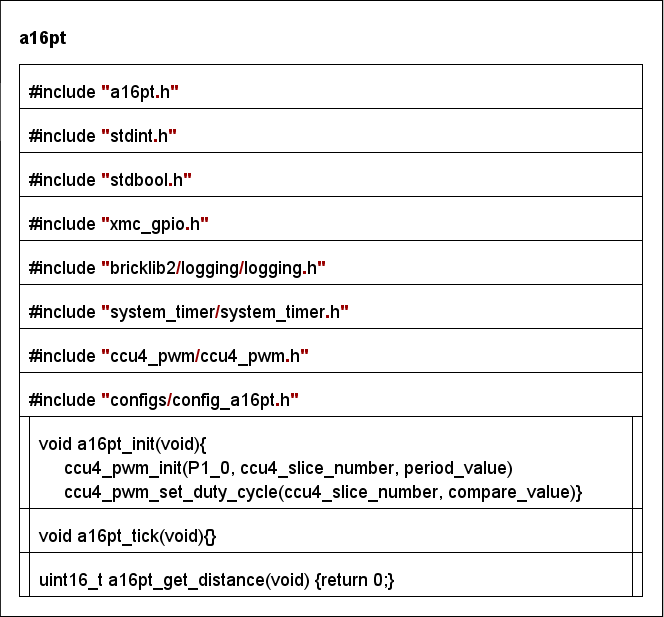
\includegraphics[width=1.0\textwidth]{Struktogramme/a16pt.png}\caption{Struktogramm der a16.pt}\label{fig:Bild2}
%\end{figure}
In der a16pt werden die für die Entfernungsmessung notwendigen Funktionen und die Interrupt anweisungen abgearbeitet, außerdem werden die Ein- und Ausgangsports hier geschaltet.\\
